%%%%%%%%%%%%%%%%%%%%%%%%%%%%%%%%%%%%%%%%%
% Large Colored Title Article
% LaTeX Template
% Version 1.1 (25/11/12)
%
% This template has been downloaded from:
% http://www.LaTeXTemplates.com
%
% Original author:
% Frits Wenneker (http://www.howtotex.com)
%
% License:
% CC BY-NC-SA 3.0 (http://creativecommons.org/licenses/by-nc-sa/3.0/)
%
%%%%%%%%%%%%%%%%%%%%%%%%%%%%%%%%%%%%%%%%%

%----------------------------------------------------------------------------------------
%	PACKAGES AND OTHER DOCUMENT CONFIGURATIONS
%----------------------------------------------------------------------------------------

\documentclass[DIV=calc, paper=a4, fontsize=11pt, twocolumn]{scrartcl}	 % A4 paper and 11pt font size

\usepackage[english]{babel} % English language/hyphenation
\usepackage[protrusion=true,expansion=true]{microtype} % Better typography
\usepackage[svgnames]{xcolor} % Enabling colors by their 'svgnames'
\usepackage[hang, small,labelfont=bf,up,textfont=it,up]{caption} % Custom captions under/above floats in tables or figures
\usepackage{booktabs} % Horizontal rules in tables
\usepackage{fix-cm}	 % Custom font sizes - used for the initial letter in the document

\usepackage{sectsty} % Enables custom section titles
\allsectionsfont{\usefont{OT1}{phv}{b}{n}} % Change the font of all section commands

\usepackage{fancyhdr} % Needed to define custom headers/footers
\pagestyle{fancy} % Enables the custom headers/footers
\usepackage{lastpage} % Used to determine the number of pages in the document (for "Page X of Total")

\usepackage{pdfpages}
% Headers - all currently empty
\lhead{}
\chead{}
\rhead{}

% Footers
\lfoot{}
\cfoot{}
\rfoot{\footnotesize Page \thepage\ of \pageref{LastPage}} % "Page 1 of 2"

\renewcommand{\headrulewidth}{0.0pt} % No header rule
\renewcommand{\footrulewidth}{0.4pt} % Thin footer rule

\usepackage{lettrine} % Package to accentuate the first letter of the text
\newcommand{\initial}[1]{ % Defines the command and style for the first letter
\lettrine[lines=3,lhang=0.3,nindent=0em]{
\color{DarkGoldenrod}
{\textsf{#1}}}{}}

%----------------------------------------------------------------------------------------
%	TITLE SECTION
%----------------------------------------------------------------------------------------

\usepackage{titling} % Allows custom title configuration

\newcommand{\HorRule}{\color{DarkGoldenrod} \rule{\linewidth}{1pt}} % Defines the gold horizontal rule around the title

\pretitle{\vspace{-30pt} \begin{flushleft} \HorRule \fontsize{50}{50} \usefont{OT1}{phv}{b}{n} \color{DarkRed} \selectfont} % Horizontal rule before the title

\title{DOMjudge at Amrita} % Your article title

\posttitle{\par\end{flushleft}\vskip 0.5em} % Whitespace under the title

\preauthor{\begin{flushleft}\large \lineskip 0.5em \usefont{OT1}{phv}{b}{sl} \color{DarkRed}} % Author font configuration

\author{Thijs Kinkhorst} % Your name

\postauthor{\footnotesize \usefont{OT1}{phv}{m}{sl} \color{Black} % Configuration for the institution name

DOMjudge team % Your institution

\par\end{flushleft}\HorRule} % Horizontal rule after the title

\date{} % Add a date here if you would like one to appear underneath the title block

%----------------------------------------------------------------------------------------

\begin{document}

\maketitle % Print the title

\thispagestyle{fancy} % Enabling the custom headers/footers for the first page 

%----------------------------------------------------------------------------------------
%	ABSTRACT
%----------------------------------------------------------------------------------------

% The first character should be within \initial{}
\initial{A}\textbf{mrita university conducted a programming contest
  with over 4000 teams participating and chose DOMjudge as the
  platform. This document describes how it was done, which problems
  were encountered and what is being done to address those.}

%----------------------------------------------------------------------------------------
%	ARTICLE CONTENTS
%----------------------------------------------------------------------------------------

\section*{Introduction}
Amrita university was in the process of organising a contest with over
4000 teams and contacted the DOMjudge team to see if our
programming contest software could scale up to this size. The DOMjudge
developers gladly took up this challenge and helped the Amrita team
design and configure a system that could handle this load.


\section*{System architecture}

The DOMjudge programming contest system provides web interfaces for
teams, jury and public, while data is stored in a database and the
back end judging system consists of daemons running on separate linux
hosts. The web interfaces are served from Apache with
a MySQL back end. It can be scaled out according to existing industry standard
best practices for these platforms, so there is no need to reinvent the wheel
for DOMjudge specifically. Indeed, the approach by the Amrita team is
based on standard web application scaling.

As front end to the system a load balancer is used, which
distributes the requests over various web servers. The public interface is
served by a Varnish cache and reads from a read-only MySQL slave, making sure
that hits on the public scoreboard do not impact the rest of the contest.
Three separate read/write webservers for the many teams and a last one for
the contest judges interact with the MySQL master read/write
database. Each webserver has two Quad core Xeon processors with 16 GB RAM.
Memcache is used both as a query cache for MySQL and as a session handler for
the team front ends. The Memory storage engine was used for the
scoreboard caching tables.

DOMjudge's judging back end, the judgehosts, scale out trivially and without
arbitrary limit; a fundamental design decision in DOMjudge. Each node has an
Intel i5 CPU and 8GB of RAM, and there were around 25 in total. All
systems were installed with Ubuntu 12.04.

A schematic overview of the setup is given on the last page of this document.

\section*{The contest}

The contest was held on 7 October 2013.  In total 4643 teams actually
participated, who made a total of 18497 submissions for the four problems.
Of those, 2453 were judged as correct. 434 teams solved at least one
problem while 100 solved all of them.

\section*{Experiences during the contest}

In preparation to the contest, it was discovered that some parts of
the web interface (like the individual scoreboard row display for each
team) could not gracefully handle the large number of teams. Drop down
select lists with thousands of elements, present in the clarification
part of the jury interface, also slowed down the browsing experience.
Some quick patches were made to disable certain non-essential
functionality in the interface.

The scoreboard was too large with over 4000 teams, so a separate
version was generated containing just the top 1000 teams. A cronjob
periodically exported this to static HTML, served to the teams and
public.

The judgehosts saw random crashes during the contests. The reason was narrowed
down to locking issues in the MySQL server, where each scoreboard cell
recalculation does a full table lock on the scoreboard cache tables.
DOMjudge does not have an active alerting system for judgehost problems,
which required quite some manual work.

Regardless of these issues, overall the contest ran smoothly.

\section*{Lessons learned and actions taken}

Overall the Amrita contest proved that DOMjudge can indeed be scaled out using
standard techniques for web application scaling, but that a few specific
bottlenecks remain when dealing with numbers of teams this large.
For one part, this is inherent in the very special nature of this contest,
and the open source aspect of DOMjudge made it possible for Amrita to
apply the local changes they required for their needs. However, we analysed
these changes to see whether it would be possible to address them in the
standard DOMjudge distribution.

On the team interface page, displaying the information relevant to the single
specific team turned out to be dependent on the total number of teams.
The cause was that calculation of the team rank involved processing
the scores of all teams in the contest. The database design has been
changed so the rank of a specific team is now cached and calculated
inside a query involving this cache table, instead of from data retrieved
from the database. Although this does not reduce the linear\footnote{%
  Most internal operations within the query are actually
  $\mathcal{O}(\log(\#\textrm{teams}))$, but due to technical details the
  overall query is still $\mathcal{O}(\#\textrm{teams})$.%
} complexity in terms of the number of teams, it reduces web server
load and the team page rendering time to be unnoticable.

For the complete scoreboard: the changes described above also impact the
time needed to compute the complete scoreboard. Discussions are ongoing
to further reduce memory usage in scoreboard calculation.
Still, a generic solution for very large contests is not yet available
at the time of writing. Aside from processing times, this is mostly a
design question, as the current table based layout does probably not
yield a useful scoreboard when it contains thousands of rows, regardless
of how fast it is calculated.

The lock contention issues in the judgedaemons has proven difficult to
reproduce and has not yet been resolved.
DOMjudge does monitor whether each of the judgedaemons checks in periodically,
but does not actively alert the administrator when a judgehost fails to do
so. Because we think that other tools already exist that do this well, we
recommend to set up external monitoring software, like Nagios, to ensure
the health of each system component is appropriately monitored.

All of the changes mentioned here have been included in DOMjudge 4.0,
which is planned to be released before the 2014 ACM ICPC world finals.

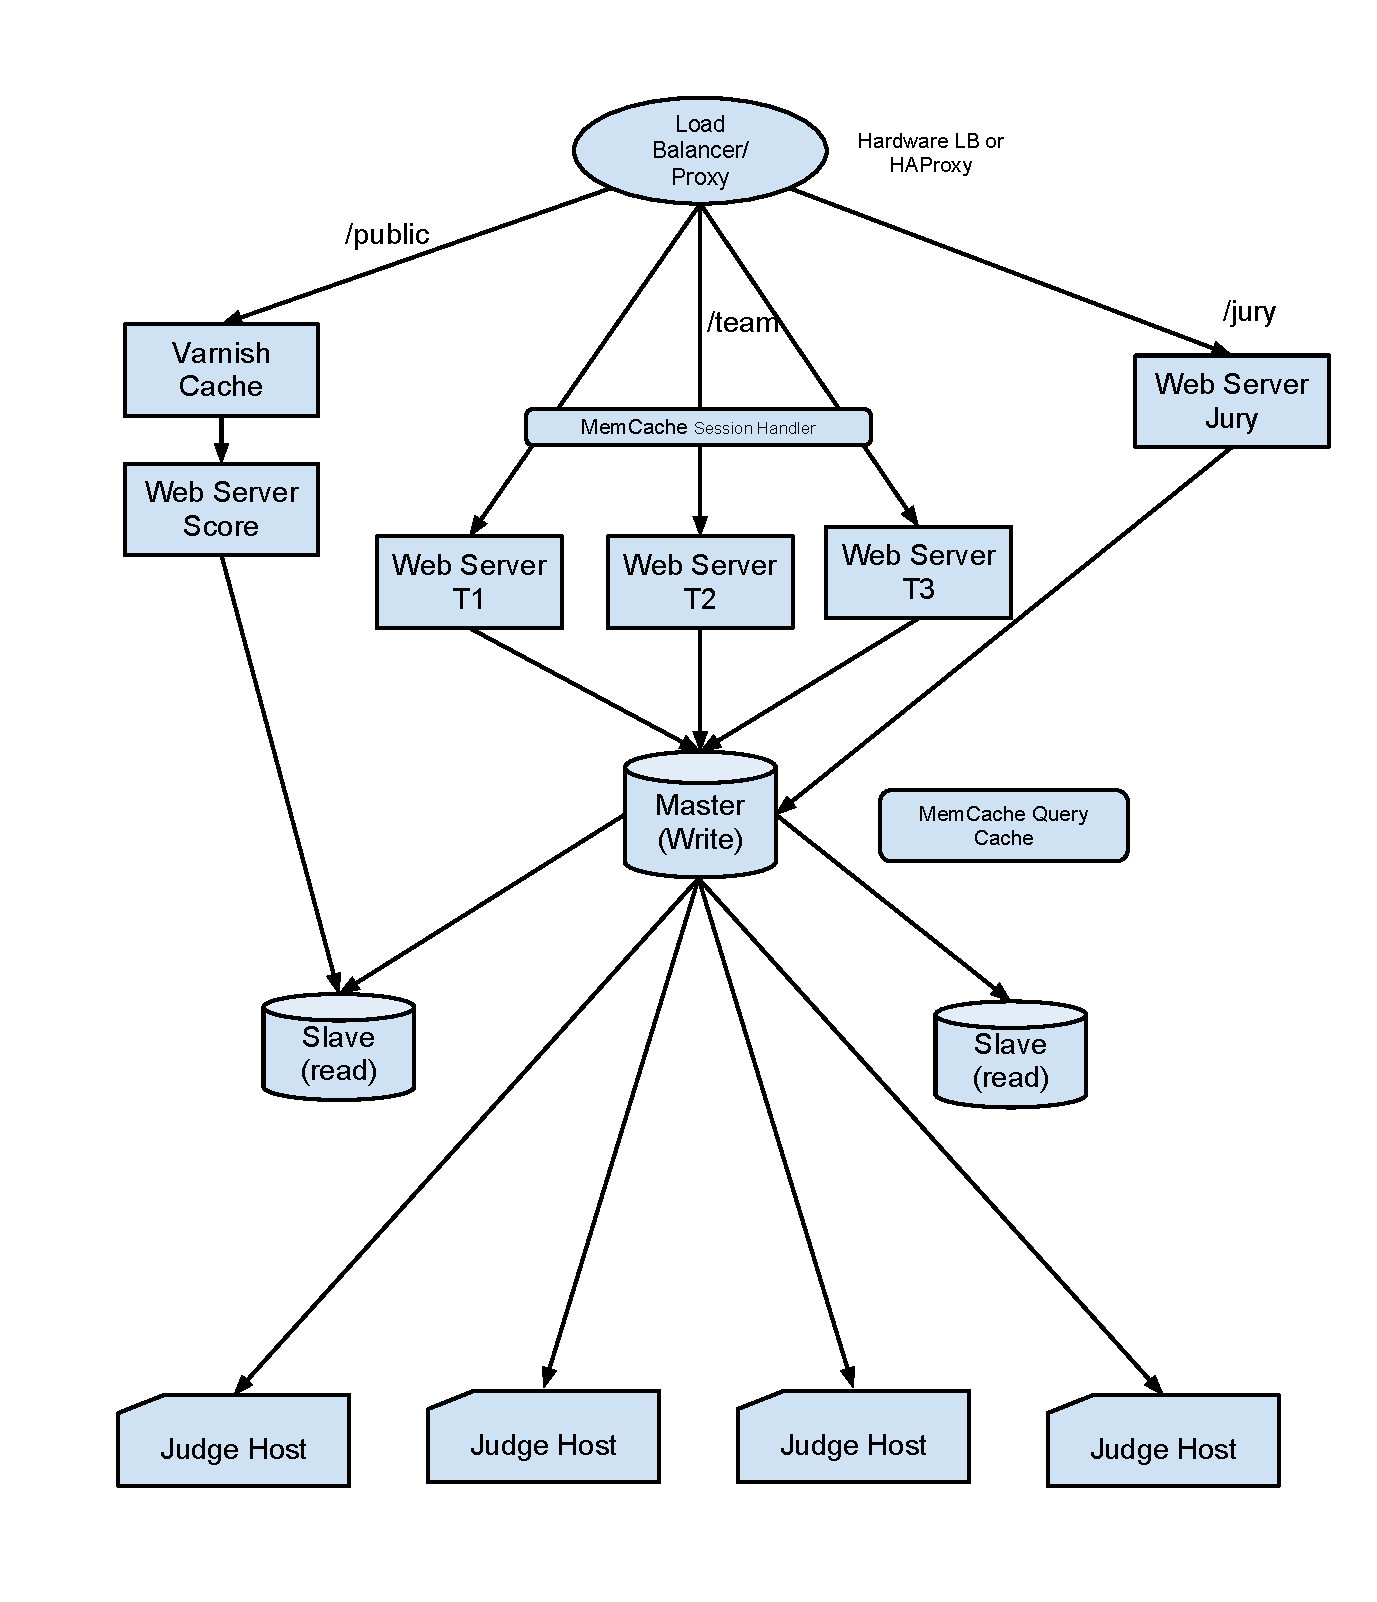
\includepdf[pages={1}]{amrita-architecture.pdf}

\end{document}
